\chapter{Hardware, Technologies and Programming Languages}


\section{Hardware}

\subsection{Raspberry Pi} 
Raspberry Pi is a series of credit card-sized single-board computers developed in the UK by the Raspberry Pi Foundation with the intention of promoting the teaching of basic computer science in schools.

\begin{wrapfigure}{r}{0.5\textwidth}
  \begin{center}
    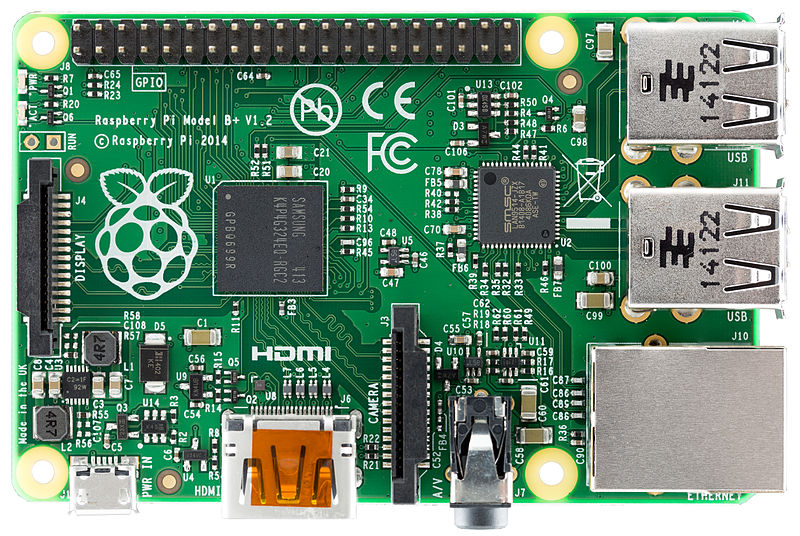
\includegraphics[width=0.5\textwidth]{./images/raspberry_pi_b.jpg}
  \end{center}
  \caption{Raspberry Pi 1 model B+}
\end{wrapfigure}

Over the past decades, computers have gotten cheaper and cheaper, so today
you can find them not only at your desk, but also in nearly every consumer
electronics device, such as smartphones and DVD players. Still, computers
aren’t so cheap that you spontaneously buy one when shopping for your
groceries. Usually, you carefully plan your next computer purchase, because
you have to use it for a couple of years.\vspace{5mm}
Computers like the Raspberry Pi will change the situation completely in the
near future. The Raspberry Pi—or Pi, for short—is a full-blown desktop PC
that costs only \$35. You can connect it directly to the Internet, and it can
display high-definition videos. Also, it runs Linux, so you don’t have to pay
for an operating system. This makes the Pi probably the first throwaway
computer in history.\vspace{5mm}
Originally, the Raspberry Foundation built the Pi to teach children how to
program, so it comes as no surprise that the Pi is an excellent device for
exactly this purpose. On top of that, you can use the Pi for many other
exciting things. For example, you can turn it into a multimedia center, use
it as a cheap but powerful web server, or play some classic games.
The Pi is also a great machine for experimenting with electronics. In contrast
to many popular microcontroller boards, such as the Arduino, the Pi runs a
full-blown operating system, and you can choose from a wide range of programming
languages to implement your projects.\vspace{5mm}
With cheap and small devices like the Raspberry Pi, a new era of ubiquitous
computing has begun, and you can be part of it. This book will help you get
up to speed quickly.\vspace{5mm}


\paragraph{Get to Know the Hardware}
Unboxing a new Pi is exciting, but it certainly is not comparable to unboxing
a new Apple product. Usually, the Pi comes in a plain cardboard box with
one or two sheets of paper containing the usual safety hints for electronic
devices and a quick-start guide.
The first version of the Pi looks attractive only to real geeks. It is a singleboard
computer without a case, and it’s the size of a credit card. It somewhat
resembles the innards of the many electronic devices you might have opened
when you were a child. Later versions of the Pi might have a case, but until
then we have to focus on its inner values, and that’s what counts, isn’t it?

\subparagraph{What’s on the Pi} 


\subsection{Car Chassis Development Kit}
  
   
\section{Technologies and Programming Languages}
\subsection{Web Application Back-End}
\subsubsection{JavaScript}
\subsubsection{NodeJs}
\subsubsection{ExpressJs}
\subsection{Web Application Front-End} 
\subsubsection{HTML (HyperText Markup Language)}
\subsubsection{CSS (Cascading Style Sheets)}
\subsubsection{Less}
\subsubsection{CoffeeScript}
\subsubsection{jQuery}
\subsection{Tools Used for Developing}
\subsubsection{Sublime Text 3}
\subsubsection{GruntJs}
\subsubsection{PuTTY}
\subsubsection{Basic UNIX commands }